%!TEX program = xelatex
\documentclass[12pt, landscape]{article}

%================ Page =================
\usepackage[
paper=letterpaper,
landscape,
left=0.20in,right=0.20in,top=1.5in,bottom=1.5in
]{geometry}

\usepackage{multicol}
\raggedcolumns
\setlength{\columnsep}{0.10in}
\setlength{\columnseprule}{0.4pt}
\setlength{\multicolsep}{0.10em}

%================ Fonts =================
\usepackage{newtxtext,newtxmath,microtype}
\let\Bbbk\relax

%================ Color =================
\usepackage[table]{xcolor}
\definecolor{sectioncolor}{RGB}{0,102,204}

%================ Lists =================
\usepackage{enumitem}
\setlist[itemize]{nosep,leftmargin=*,itemsep=0pt,topsep=0pt}
\setlist[enumerate]{nosep,leftmargin=*,itemsep=0pt,topsep=0pt}

%================ Sections =================
\usepackage{titlesec}
\titleformat{\section}{\bfseries\color{sectioncolor}\large}{}{0pt}{}
\titlespacing*{\section}{0pt}{0.25ex}{0.25ex}
\setcounter{secnumdepth}{0}

%================ Math =================
\usepackage{amsmath,amssymb,bm}
\usepackage{mathtools}

%================ Optional visuals =================
\usepackage{tikz}
\usetikzlibrary{arrows.meta,calc}

%================ Global =================
\pagestyle{empty}
\setlength{\parindent}{0pt}
\setlength{\parskip}{0pt}
\linespread{0.95}
\makeatletter
\g@addto@macro\normalsize{\bfseries\boldmath}
\makeatother

%================ Macros =================
\newcommand{\vct}[1]{\bm{#1}}
\newcommand{\uvct}[1]{\bm{\hat{#1}}}
\newcommand{\norm}[1]{\left\lVert#1\right\rVert}
\newcommand{\abs}[1]{\left\lvert#1\right\rvert}
\newcommand{\dotp}{\!\cdot\!}
\newcommand{\grad}{\nabla}
\newcommand{\pd}[2]{\frac{\partial #1}{\partial #2}}
\newcommand{\pdd}[2]{\frac{\partial^2 #1}{\partial #2^2}}
\newcommand{\comp}[1]{\mathrm{comp}_{#1}}
\newcommand{\proj}[1]{\mathrm{proj}_{#1}}

\begin{document}
\vspace*{\fill}
	
	{\Large\bfseries Math 281 Final Concept Sheet --- Master Workflows}\par
	\vspace{-0.35em}\hrule\vspace{0.18em}
	
	\begin{multicols}{3}
		\raggedright
		
		\section{Master Router (Fast Recognition)}
		\begin{itemize}
			\item \textbf{Sphere / quadric / plane / line / distance?} Use geometry formulas.
			\item \textbf{Vector curve?} Differentiate componentwise. Speed $=\norm{\vct r'}$, length $=\int \norm{\vct r'}dt$.
			\item \textbf{Limit in 2 vars?} Test \textbf{two paths}. Same lines does \textbf{not} prove existence.
			\item \textbf{First/Second partials?} Differentiate carefully. Keep mixed terms straight.
			\item \textbf{Chain rule / $du$ / related rates?} Write base formula first, then differentiate.
			\item \textbf{Intersection curve tangent?} Use \textbf{$\grad F\times\grad G$} for tangent direction.
			\item \textbf{Tangent plane / normal line?} Separate \textbf{$z=f(x,y)$} from \textbf{$F(x,y,z)=c$}.
			\item \textbf{Directional derivative / max rate?} $\grad f$, normalize direction, then dot product.
			\item \textbf{Local extrema?} Solve $f_x=f_y=0$, then second derivative test.
			\item \textbf{Absolute extrema on closed region?} Interior crit pts + every boundary + endpoints.
			\item \textbf{Constraint given?} Use \textbf{Lagrange multipliers}: $\grad f=\lambda \grad g$.
		\end{itemize}
		
		\textbf{Exam Strategy:} Label the type first. Do not start computing blindly. Use the shortest valid route. If a line-path already gives parameter-dependent answer, stop. For optimization, write the full pipeline every time. For geometry, normals and direction vectors are everything.
		
		\section{Geometry, Lines, Planes (Ch.12)}
		\textbf{Vector basics:} $\norm{\vct u}=\sqrt{u_1^2+u_2^2+u_3^2}$, $\uvct u=\vct u/\norm{\vct u}$.\\
		\textbf{Dot:} $\vct u\dotp\vct v=u_1v_1+u_2v_2+u_3v_3$, \quad $\cos\theta=\dfrac{\vct u\dotp\vct v}{\norm{\vct u}\norm{\vct v}}$.
		\begin{itemize}
			\item \textbf{Orthogonal}: $\vct u\dotp\vct v=0$ \quad \textbf{Parallel}: $\vct u=\lambda \vct v$
			\item \textbf{Scalar comp of $\vct b$ along $\vct a$}: $\comp{\vct a}\vct b=\dfrac{\vct b\dotp\vct a}{\norm{\vct a}}$
			\item \textbf{Proj of $\vct b$ onto $\vct a$}: $\proj{\vct a}\vct b=\dfrac{\vct b\dotp\vct a}{\norm{\vct a}^2}\vct a$
		\end{itemize}
		
		\textbf{Cross:} $\norm{\vct u\times\vct v}=\norm{\vct u}\norm{\vct v}\sin\theta$
		\begin{itemize}
			\item parallelogram area $=\norm{\vct u\times\vct v}$
			\item triangle area $=\frac12\norm{\vct u\times\vct v}$
			\item normal to plane from 3 points: $(B-A)\times(C-A)$
		\end{itemize}
		
		\textbf{Triple product:} $V=\abs{\vct a\dotp(\vct b\times\vct c)}$ gives parallelepiped volume.
		
		\textbf{Lines:} $\vct r(t)=\vct r_0+t\vct d$\\
		Parametric: $x=x_0+at,\ y=y_0+bt,\ z=z_0+ct$\\
		Symmetric: $\frac{x-x_0}{a}=\frac{y-y_0}{b}=\frac{z-z_0}{c}$ (if comp is 0, keep constant)
		
		\textbf{Planes:} Vector: $\vct n\dotp(\langle x,y,z\rangle-\langle x_0,y_0,z_0\rangle)=0$\\
		Scalar: $Ax+By+Cz=D$ with normal $\vct n=\langle A,B,C\rangle$.
		
		\textbf{Distance Formulas:}
		\begin{itemize}
			\item Point to plane: $d=\frac{\abs{Ax_0+By_0+Cz_0-D}}{\sqrt{A^2+B^2+C^2}}$
			\item Point to line thru $A,B$: $d=\frac{\norm{(P-A)\times(B-A)}}{\norm{B-A}}$
			\item Parallel planes $D_1,D_2$: $d=\frac{\abs{D_2-D_1}}{\sqrt{A^2+B^2+C^2}}$
			\item Skew lines ($L_1: \vct a+t\vct u$, $L_2: \vct b+s\vct v$):\\ $d=\frac{\abs{(\vct b-\vct a)\dotp(\vct u\times\vct v)}}{\norm{\vct u\times\vct v}}$. If $\vct u\times\vct v=\vct 0$, use point-to-line.
		\end{itemize}
		
		\textbf{Ch. 12 Checklists:}
		\begin{itemize}
			\item \textbf{Sphere from center + point:} $(x-a)^2+(y-b)^2+(z-c)^2=r^2$, $r=$ distance to point.
			\item \textbf{Plane thru 3 points:} form two dir vectors $\to$ cross for normal $\to$ plug point into point-normal form.
			\item \textbf{Plane thru point containing line:} line gives one dir vector $\to$ point on line to given point gives second $\to$ cross for normal.
			\item \textbf{Line-plane intersection:} plug line parametrics into plane $\to$ solve for parameter $\to$ substitute back.
			\item \textbf{Parallel / skew lines:} compare dir vectors $\to$ if not parallel, solve simultaneously. No common point = skew.
			\item \textbf{Angle between planes:} $\cos\theta=\frac{\vct n_1\dotp \vct n_2}{\norm{\vct n_1}\norm{\vct n_2}}$. Use acute.
		\end{itemize}
		
		\textbf{Surface ID / Quadratic Surfaces:}
		\begin{itemize}
			\item \textbf{Missing variable} $\Rightarrow$ cylinder in that direction
			\item sphere: $(x-a)^2+(y-b)^2+(z-c)^2=r^2$
			\item ellipsoid: $\dfrac{x^2}{a^2}+\dfrac{y^2}{b^2}+\dfrac{z^2}{c^2}=1$
			\item elliptic paraboloid: $z=ax^2+by^2+k$
			\item hyperbolic paraboloid: $z=ax^2-by^2+k$
			\item 1-sheet hyperboloid: $+,+,-=1$
			\item 2-sheet hyperboloid: $+,-,-=1$
			\item cone: $z^2=ax^2+by^2$
		\end{itemize}
		\textbf{Fast ID tool:} set $x=c$, $y=c$, $z=c$ and inspect traces.
		
		\section{Vector Curves (Ch.13)}
		\textbf{Space curve:} $\vct r(t)=\langle x(t),y(t),z(t)\rangle$.\\
		\textbf{Velocity:} $\vct v=\vct r'(t)$ \quad \textbf{Accel:} $\vct a=\vct r''(t)$ \quad \textbf{Speed:} $\norm{\vct r'(t)}$\\
		\textbf{Rules:} $(c\vct u)'=c\vct u'$, $(\vct u\dotp\vct v)'=\vct u'\dotp\vct v+\vct u\dotp\vct v'$, $(\vct u\times\vct v)'=\vct u'\times\vct v+\vct u\times\vct v'$
		
		\textbf{Ch. 13 Checklists:}
		\begin{itemize}
			\item \textbf{Domain/Limit:} intersect domains / componentwise limits.
			\item \textbf{Curve length:} compute $\vct r'(t)$ $\to$ compute $\norm{\vct r'(t)}$ $\to$ integrate $\int_a^b \norm{\vct r'(t)}\,dt$.
			\item \textbf{Reparametrize:} compute speed $\to$ integrate to get $s(t)$ $\to$ invert to get $t(s)$ $\to$ substitute into $\vct r(t)$.
			\item \textbf{Curve ID:} Line? All components affine (linear). Parabola? One quadratic, another linear. Intersection? Parameterize easy piece first.
		\end{itemize}
		
		\textbf{Tangent, Normal, Binormal, Curvature:}
		\[
		\vct T=\frac{\vct r'}{\norm{\vct r'}},\qquad \vct N=\frac{\vct T'}{\norm{\vct T'}},\qquad \vct B=\vct T\times \vct N
		\]
		\[
		\kappa=\frac{\norm{\vct T'}}{\norm{\vct r'}}=
		\frac{\norm{\vct r'\times \vct r''}}{\norm{\vct r'}^3}
		\]
		\textbf{Curvature Checklists:}
		\begin{itemize}
			\item Curve $y=f(x)$: $\kappa=\frac{\abs{f''(x)}}{(1+[f'(x)]^2)^{3/2}}$
			\item Parametric: $\kappa=\frac{\abs{x'y''-y'x''}}{(x'^2+y'^2)^{3/2}}$
		\end{itemize}
		
		\begin{itemize}
			\item \textbf{Osculating plane}: normal $\vct B$. Checklist: compute $\vct r',\vct r''$ $\to$ find $\vct B\parallel \vct r'\times \vct r''$ $\to$ use point-normal plane eq.
			\item \textbf{Normal plane}: normal vector $\vct T$
			\item \textbf{Osculating circle}: same tangent, normal, curvature, radius $=1/\kappa$
		\end{itemize}
		
		\textbf{Acceleration Decomposition:}
		$a_T=\frac{\vct v\dotp \vct a}{\norm{\vct v}},\qquad a_N=\sqrt{\norm{\vct a}^2-a_T^2}$.\\
		\textbf{Meaning:} $a_T$ changes speed, $a_N$ bends path.
		
		\section{Limits, Partials, Rates (Ch.14)}
		\textbf{Limits in 2 vars:} To show DNE, pick two paths with diff answers.
		\begin{itemize}
			\item start with \textbf{lines}: $y=mx$
			\item then try \textbf{curved paths}: $y=x^2,\ y=kx^2,\ x=y^2$
			\item polar helps when expression has $x^2+y^2$
		\end{itemize}
		\textbf{Patterns:} If denom has $xy$, test $y=x$ and $y=-x$. If denom has $x^2+y^2$, compare num order. If polar gives leftover $\theta$, DNE.\\
		\textbf{Example:} $\frac{2xy}{x^2+2y^2} \to$ try $y=mx \to \frac{2x(mx)}{x^2+2m^2x^2}=\frac{2m}{1+2m^2}$. Depends on $m$, so \textbf{DNE} (Limit cue: if result depends on $m$, limit DNE immediately).
		
		\textbf{Continuity \& Linearization:}
		Continuous if limit exists and equals function value.\\
		Differentiable means locally approximated by a linear map: $f(a+\Delta x,b+\Delta y)\approx f(a,b)+f_x\Delta x+f_y\Delta y$.\\
		Linearization: $L(x,y)=f(a,b)+f_x(a,b)(x-a)+f_y(a,b)(y-b)$
		
		\textbf{Second Partials + Clairaut:} keep first partials easy to differentiate. Clairaut: if continuous nearby, $f_{xy}=f_{yx}$.\\
		\textbf{Example:} $f(x,y)=4x^3-xy^2 \Rightarrow f_x=12x^2-y^2,\ f_y=-2xy \Rightarrow f_{xx}=24x,\ f_{xy}=-2y,\ f_{yx}=-2y,\ f_{yy}=-2x$.
		
		\textbf{Differentials:} $du=u_x\,dx+u_y\,dy$\\
		\textbf{Example:} $u=\ln(1+se^{2t}) \Rightarrow du=\frac{1}{1+se^{2t}}\left(e^{2t}\,ds+2se^{2t}\,dt\right)$
		
		\textbf{Chain Rule Checklist:} compute $f_x,f_y,f_z$ $\to$ compute $x',y',z'$ $\to$ substitute all expressions.\\
		$\frac{du}{dp}=f_x\frac{dx}{dp}+f_y\frac{dy}{dp}+f_z\frac{dz}{dp}$.
		
		\textbf{Implicit Differentiation:}
		If $F(x,y)=0$, $\frac{dy}{dx}=-\frac{F_x}{F_y}$.
		For surface $F(x,y,z)=0$, $z_x=-\frac{F_x}{F_z}$, $z_y=-\frac{F_y}{F_z}$.
		
		\textbf{Related rates:} write physical formula first, then differentiate in time. \textbf{Do not plug numbers until after differentiating.}\\
		\textbf{Example:} $A=\frac12xy\sin\theta \Rightarrow \frac{dA}{dt}=\frac12\left(y\sin\theta\frac{dx}{dt} +x\sin\theta\frac{dy}{dt} +xy\cos\theta\frac{d\theta}{dt}\right)$.
		
		\section{Gradients, Tangents, Normals}
		\textbf{Gradient \& Directional Derivative:}
		$D_{\uvct u}f(P)=\grad f(P)\dotp \uvct u$.\\
		\textbf{Checklist:} compute gradient $\to$ eval at point $\to$ make direction unit length $\to$ dot product. Toward point $Q$ from $P$: use $Q-P$. \textbf{Example:} from $(-2,0)$ toward $(2,-3)$ use direction $\langle 4,-3\rangle$, then divide by $5$.
		
		\textbf{Max Rate:} $\max D_{\uvct u}f=\norm{\grad f}$.
		Direction of max inc = $\grad f/\norm{\grad f}$. Max dec = $-\grad f/\norm{\grad f}$.\\
		\textbf{Example:} Max inc of $f(x,y,z)=ze^{xy}$ at $(0,1,2)$. $\grad f=\langle zye^{xy},zxe^{xy},e^{xy}\rangle$. Evaluate first. Exam trap: direction = vector, rate = magnitude.
		
		\textbf{Tangent vs Normal Quick Split:}
		\begin{itemize}
			\item \textbf{Tangent plane to surface}: plane that touches surface locally
			\item \textbf{Normal line to surface}: line perpendicular to tangent plane
			\item \textbf{Tangent line to curve}: line in curve direction
			\item \textbf{Normal plane to curve}: plane perpendicular to tangent line
		\end{itemize}
		
		\textbf{For graph $z=f(x,y)$ at $(a,b,z_0)$:}
		\begin{itemize}
			\item Tangent plane: $z-z_0=f_x(a,b)(x-a)+f_y(a,b)(y-b)$
			\item Normal vector: $\langle f_x(a,b),f_y(a,b),-1\rangle$
			\item Normal line: $(x,y,z)=(a,b,z_0)+t\langle f_x(a,b),f_y(a,b),-1\rangle$
		\end{itemize}
		
		\textbf{For level surface $F(x,y,z)=c$ at $P$:}
		\begin{itemize}
			\item Tangent plane: $\grad F(P)\dotp\langle x-x_0,y-y_0,z-z_0\rangle=0$
			\item Normal vector: $\grad F(P)$
			\item Normal line: $(x,y,z)=P+t\,\grad F(P)$
		\end{itemize}
		
		\textbf{Review cue:} $z=3x^2-y^2+2x$ and $z=e^x\cos y$ are \textbf{graph form}. $x^2+2y^2-3z^2=3$, $xy+yz+zx=3$, and $\sin(xyz)=x+2y+3z$ are \textbf{level surfaces}.
		
		\textbf{Parallel tangent plane prob:} If tang plane to $F=c$ is parallel to $Ax+By+Cz=D$, normals are parallel: $\grad F(P)=\lambda \langle A,B,C\rangle$. Solve with surface equation.\\
		\textbf{Example:} $x^2+4y^2-z^2=4$, plane $2x+2y+z=5$. Set $\grad F=\langle 2x,8y,-2z\rangle=\lambda\langle 2,2,1\rangle$, plug into surface.
		
		\textbf{Intersection tangent line:}
		If curve is intersection of $F=0$ and $G=0$, then tangent direction is
		\[
		\vct d=\grad F(P)\times \grad G(P)
		\]
		So tangent line is
		\[
		(x,y,z)=P+t\,\vct d
		\]
		\textbf{Example:} surface $z=2x^2-y^2$ and plane $z=4$. Rewrite as $F=z-2x^2+y^2$, $G=z-4$. Cross product at point.
		
		\section{Optimization}
		\textbf{Local Extrema Checklist:} solve $f_x=f_y=0$ $\to$ compute $f_{xx},f_{yy},f_{xy}$ $\to$ classify with $D=f_{xx}f_{yy}-(f_{xy})^2$.
		\begin{itemize}
			\item $D>0, f_{xx}>0$: min \quad $D>0, f_{xx}<0$: max
			\item $D<0$: saddle \quad $D=0$: inconclusive
		\end{itemize}
		Exam trap: solve system completely, don't stop at one point.
		
		\textbf{Absolute Extrema Checklist:} interior crit points $\to$ reduce each boundary to one var $\to$ compare all values.\\
		\textbf{Example Triangle} $(0,0),(0,6),(6,0)$: edge 1 ($x=0$), edge 2 ($y=0$), edge 3 ($x+y=6$). Sub into $f$, solve 1-var extrema.\\
		\textbf{Example Disk} $x^2+y^2\le 4$: interior ($f_x=f_y=0$), boundary (use $x=2\cos t,\ y=2\sin t$ or $x^2+y^2=4$).
		
		\textbf{Closed / Bounded / EVT:}
		\begin{itemize}
			\item \textbf{Closed set}: contains boundary points
			\item \textbf{Bounded set}: fits inside some large disk/ball
			\item \textbf{EVT}: continuous on closed and bounded set $\Rightarrow$ absolute max/min exist
		\end{itemize}
		
		\textbf{Lagrange Multiplier Method:}
		\[
		\grad f=\lambda \grad g,\qquad g=c
		\]
		2-variable form:
		\[
		f_x=\lambda g_x,\qquad f_y=\lambda g_y,\qquad g(x,y)=c
		\]
		3-variable form:
		\[
		f_x=\lambda g_x,\quad f_y=\lambda g_y,\quad f_z=\lambda g_z,\quad g(x,y,z)=c
		\]
		Solve all together, then compare values of $f$ at all candidate points.
		
		\section{Fact / Traps / T/F Bank}
		\textbf{Algebra \& Exam Traps:}
		\begin{itemize}
			\item normalize direction vectors
			\item do not lose minus signs in $f_{xy}$
			\item for level surfaces, point must satisfy surface first
			\item for tangent plane parallelism, compare \textbf{normals}
			\item for closed regions, boundaries matter
			\item when plugging line into plane, solve parameter carefully
		\end{itemize}
		
		\textbf{Tiny Vocab Facts:}
		\begin{itemize}
			\item \textbf{Normal vector} is perp to a plane or tangent plane.
			\item \textbf{Tangent vector} points along a curve: $\vct r'(t)$.
			\item \textbf{Normal vector to level surface} $F=c$ is $\grad F$.
			\item \textbf{Normal plane} to a curve has normal $\vct T$.
			\item \textbf{Osculating plane} to a curve has normal $\vct B$.
			\item \textbf{Critical point}: where $\grad f=\vct 0$ or partials DNE.
		\end{itemize}
		
		\textbf{False unless special case:}\\
		$\abs{\vct u+\vct v}=\abs{\vct u}+\abs{\vct v}$, \quad
		$\abs{\vct u\dotp\vct v}=\abs{\vct u}\abs{\vct v}$, \quad
		$\abs{\vct u\times\vct v}=\abs{\vct u}\abs{\vct v}$, \quad
		$\vct u\times\vct v=\vct v\times\vct u$, \quad
		$\vct u\times(\vct v\times\vct w)=(\vct u\times\vct v)\times\vct w$, \quad
		if $f_x,f_y$ exist then $f$ diff, \quad
		if all line-path limits agree then full limit exists.
		
		\textbf{True core facts:}\\
		$\vct u\dotp(\vct v\times\vct w)=(\vct u\times\vct v)\dotp\vct w$, \quad
		$(\vct u\times\vct v)\dotp \vct u=0$, \quad
		Cauchy-Schwarz: $\abs{\vct u\dotp\vct v}\le \norm{\vct u}\norm{\vct v}$, \quad
		if $\norm{\vct r(t)}=1$, then $\vct r\dotp\vct r'=0$, \quad
		if $\kappa(t)=0$ for all $t$, curve is a line.
		
		\vspace{0.3em}
		\begin{center}
			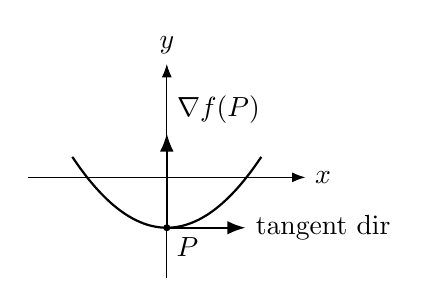
\begin{tikzpicture}[scale=0.8,>=Latex]
				\draw[->] (-2.2,0) -- (2.2,0) node[right] {$x$};
				\draw[->] (0,-1.6) -- (0,1.8) node[above] {$y$};
				\draw[smooth, thick] plot[domain=-1.5:1.5] (\x,{0.5*(\x*\x)-0.8});
				\fill (0,-0.8) circle (1.6pt) node[below right] {$P$};
				\draw[->,thick] (0,-0.8) -- (0,0.7) node[above right] {$\grad f(P)$};
				\draw[->,thick] (0,-0.8) -- (1.25,-0.8) node[right] {tangent dir};
			\end{tikzpicture}
			\quad
			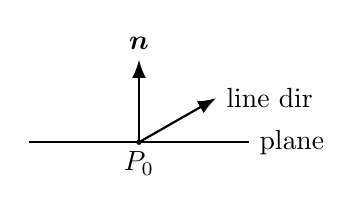
\begin{tikzpicture}[scale=0.7,>=Latex]
				\draw[thick] (-2,0) -- (2,0) node[right] {plane};
				\fill (0,0) circle (1.4pt) node[below] {$P_0$};
				\draw[->,thick] (0,0) -- (0,1.5) node[above] {$\vct n$};
				\draw[->,thick] (0,0) -- (1.4,0.8) node[right] {line dir};
			\end{tikzpicture}
		\end{center}
		
	\textbf{Parameterization Quick Guide}
	
	\textbf{Line through point $P$ with direction $\vct d$:}  
	$(x,y,z)=P+t\,\vct d$.  
	Example: through $(1,2,3)$ dir $\langle2,-1,4\rangle$:  
	$x=1+2t,\ y=2-t,\ z=3+4t$.
	
	\textbf{Circle / cylinder ($x^2+y^2=r^2$):}  
	Use $x=r\cos t,\ y=r\sin t$.
	
	\textbf{Ellipse ($x^2/a^2+y^2/b^2=1$):}  
	Use $x=a\cos t,\ y=b\sin t$.
	
	\textbf{Intersection curve recipe:}  
	1. Parameterize the easier equation (often a circle).  
	2. Let $t$ be the parameter.  
	3. Substitute into the other equation.
	
	Example: $x^2+y^2=16$, $x+z=5$.  
	Use $x=4\cos t,\ y=4\sin t$.  
	Then $z=5-4\cos t$.
	
	\textbf{Tangent line to intersection of surfaces $F=0$, $G=0$:}  
	Direction $=\grad F\times\grad G$.  
	Line: $(x,y,z)=P+t(\grad F\times\grad G)$.
	
	\end{multicols}
	\vspace*{\fill}
	
\end{document}